\newpage
\section{Auswertung}
\subsection{Ablenkung des Elektronenstrahls im E-Feld}
Die im Versuch gemessenen Werte sind in Tabelle \ref{tab:U} zu finden.
\begin{table}[H]
  \centering
  \caption{Gemessene Spannung bei unterschiedlicher Auslenkung}
  \label{tab:U}
  \sisetup{table-format=2.1}
\begin{tabular}{S[table-format=3.1] S S S S S S}
    \toprule
     & \multicolumn{5}{c}{Spannung ($\symup{U_d}$ / V)} \\
\cmidrule(lr){2-6}
    {Auslenkung (D/ Zoll)} & {bei 230V}
    &   {bei 250V}
     &  {bei 300V}
     &  {bei 350V}
     &  {bei 400V}\\
    \midrule
    0    & -24,3 & -26,5 & -30,6 & &\\
    0,25 & -19,3 & -22   & -25,1 & -30,7 & -34,2\\
    0,5  & -15   & -17,5 & -21   & -23,5 & -27,6\\
    0,75 & -11,5 & -12,7 & -14,8 & -17,74& -19,84\\
    1    & -7,4  & -8,1  & -9,6  & -12,34& -12,31\\
    1,25 & -3,5  & -3,55 & -4,45 & -5,7  & -4,82\\
    1,5  & 0,38  & 0,88  & 1,52  & 1,46  & 2,4\\
    1,75 & 5,04  & 6,44  & 7,24  & 7,76  & 10,3\\
    2    & 9,46  & 10,85 & 12,88 & 14,3  & 18\\
    \bottomrule
  \end{tabular}
\end{table}
Zunächst wird der Abstand gegen die Spannung aufgetragen.
Dafür werden die Angaben des Abstandes in Meter %$\mathrm{m}$
umgerechnet.
Der ermittelte umrechnugsfaktor beträgt \\
 0,0252 $\mathrm{m/Zoll}$ .
Die entstandenen Graphen sind in den Abbildungen \ref{fig:230b} - \ref{fig:400b} zu sehen.

\begin{figure}[H]
\centering
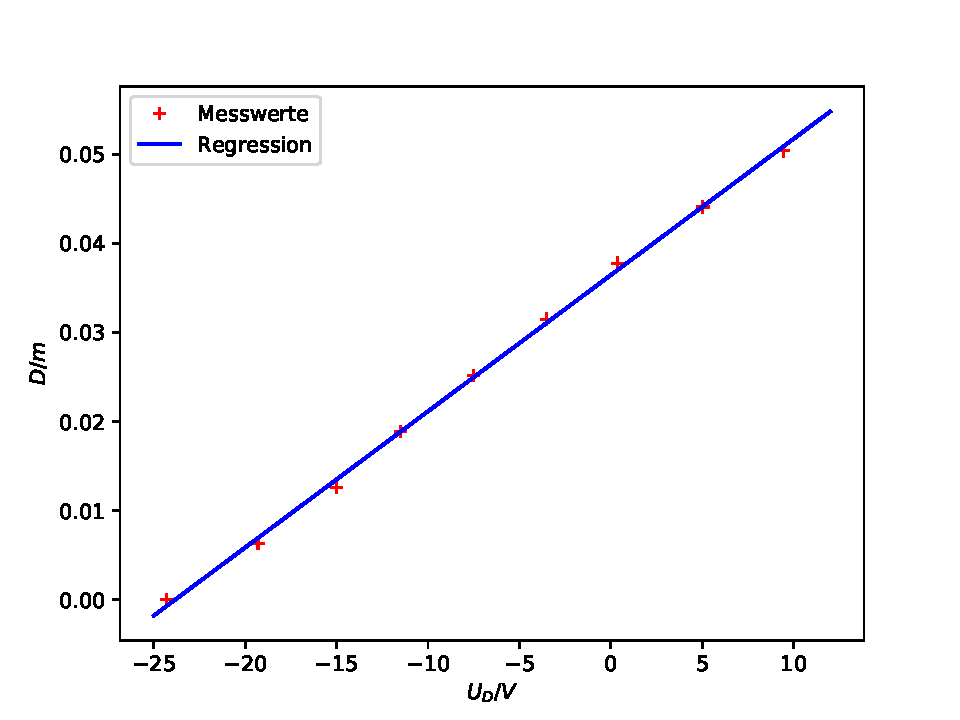
\includegraphics[height=9cm]{plot230b.pdf}
\caption{Empfindlichkeit für 230V}
\label{fig:230b}
\end{figure}
\begin{figure}[H]
\centering
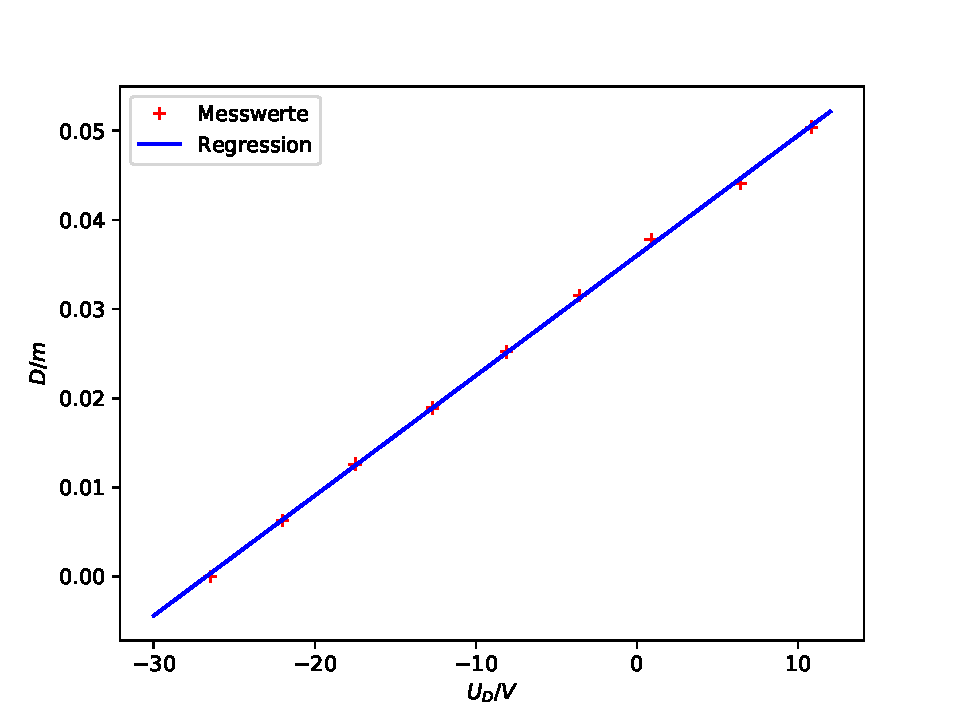
\includegraphics[height=9cm]{plot250b.pdf}
\caption{Empfindlichkeit für 250V}
\label{fig:250b}
\end{figure}
\begin{figure}[H]
\centering
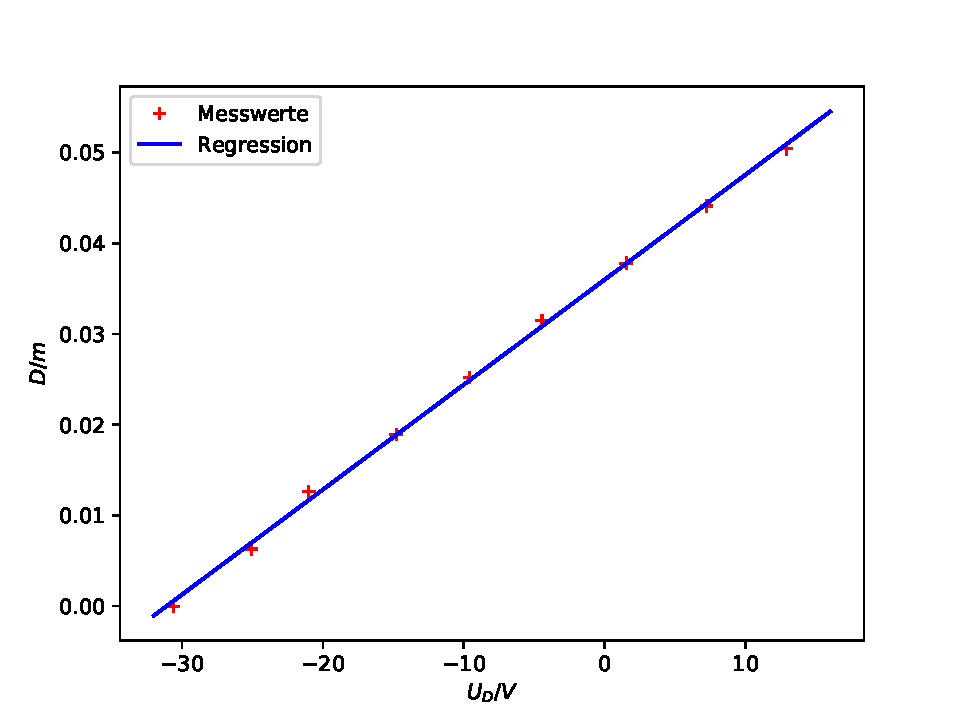
\includegraphics[height=9cm]{plot300b.pdf}
\caption{Empfindlichkeit für 300V}
\label{fig:300b}
\end{figure}
\begin{figure}[H]
\centering
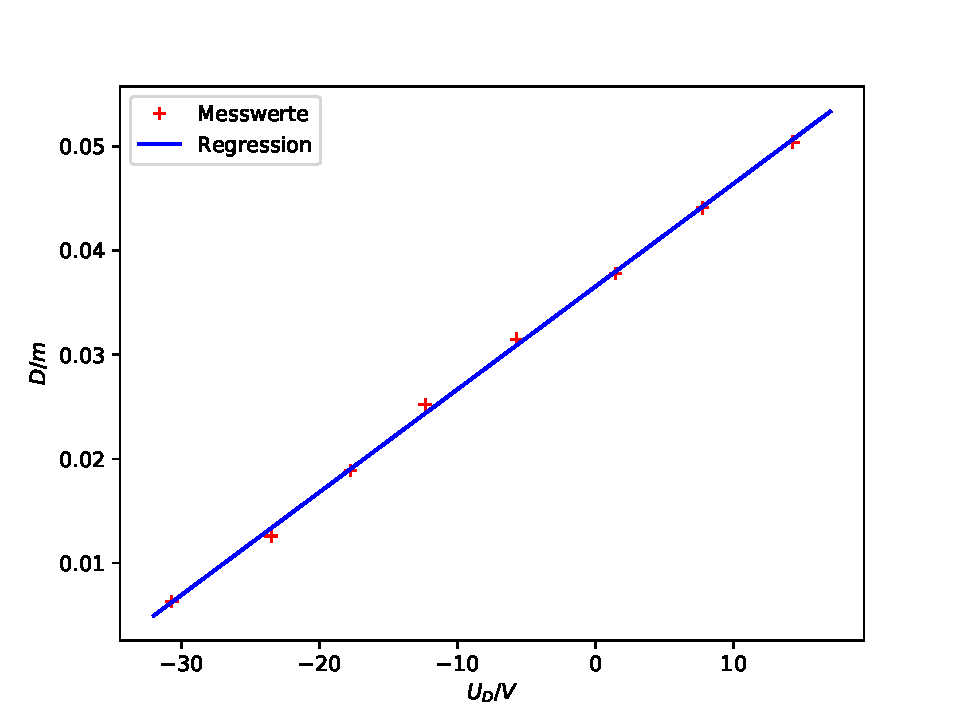
\includegraphics[height=9cm]{plot350b.pdf}
\caption{Empfindsamkeit für 350V}
\label{fig:350b}
\end{figure}
\begin{figure}[H]
\centering
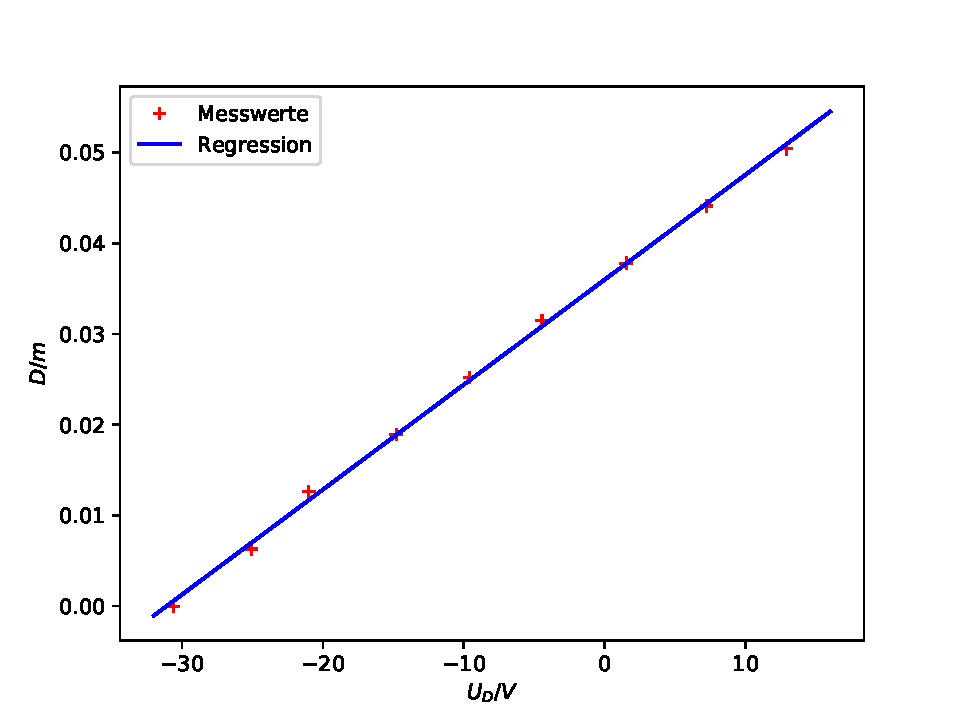
\includegraphics[height=9cm]{plot300b.pdf}
\caption{Empfindlichkeit für 400V}
\label{fig:400b}
\end{figure}

Aus Gleichung (\ref{eqn:dud}) folgt ein linearer Zusammenhang zwischen D und $\symup{U_d}$.
Somit folgt eine lineare Ausgleichsrechnung mit
\begin{equation*}
  D(U_d) = U_d\cdot a +b
\end{equation*}
Die Steigung a entspricht hierbei der Empfindlichkeit $\sfrac{D}{U_d}$ für die unterschiedlichen Beschleunigungsspannungen.
Die Parameter a und b sind in Tabelle \ref{tab:empf} aufgelistet.
\begin{table}[H]
  \centering
  \caption{Parameter der Regression}
  \label{tab:empf}
  \begin{tabular}{c c c}
    \toprule
    $ \symup{Beschleunigungsspannung \, U_B}\,/\, \mathrm{V} $ & $\symup{C_{empf.}} = a = \frac{D}{U_d}\, / \,(\mathrm{\frac{N}{C}})$ & b/ $\, \mathrm{m}$ \\
    \midrule
    230 & $ (0,001530 \pm 0,000020) $&$ (0,001530 \pm 0,000020)$ \\
    250 & $ (0,001346 \pm 0,000010) $&$ (0,001346 \pm 0,000010)$\\
    300 & $ (0,001157 \pm 0,000014) $&$ (0,001157 \pm 0,000014)$ \\
    350 & $ (0,000987 \pm 0,000013) $&$ (0,000987 \pm 0,000013)$ \\
    400 & $ (0,000841\pm 0,000006)  $&$ (0,000841 \pm 0,000006)$  \\
    \bottomrule
  \end{tabular}
\end{table}
Im Folgenden wird die Empfindlichkeit gegen $\sfrac{1}{U_B}$ aufgetragen.
Dies ist in Abbildung \ref{fig:empfvsu} zu sehen.

\begin{figure}[H]
\centering
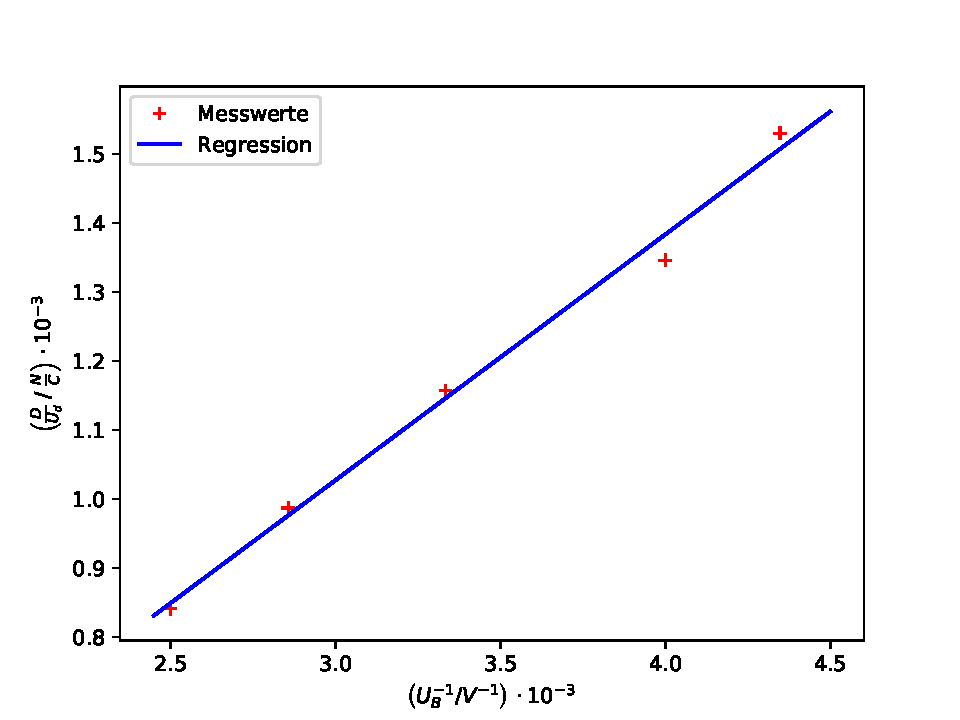
\includegraphics[width=\textwidth]{empfvsu.pdf}
\caption{Empfindlichkeit gegen $1/U_B$}
\label{fig:empfvsu}
\end{figure}
Es wurde ebenfalls eine lineare Ausgleichsrechnung durchgeführt.
Die Formel lautet:
\begin{equation*}
  \frac{1}{U_b}\left(\frac{D}{U_d}\right) = a \cdot \frac{D}{U_d} +b
\end{equation*}
Die ermittelten Parameter betragen
\begin{align*}
  C_{Messung} = a &= (0,356\pm 0,018)\, \mathrm{m}\\
  b  &= (-0.04\pm 0.06)\, \mathrm{\frac{N}{C}}.
\end{align*}
Nun wird die Größe
\begin{equation}
  C_{Theorie} = \frac{pL}{2d}
  \label{eqn:a}
\end{equation}
berechnet.
Diese drei Größen werden aus der Anleitung entnommen.
Dabei ist p die Länge der Ablenkplatten, d der Abstand der beiden Platten und L der Abstand der Platten zum Leuchtschirm.
Die Größe d wird über die beiden Angaben in der Anleitung gemittelt.
\begin{align}
  p &= 1,9\, \mathrm{cm} \\
  d &= (0,665 \pm 0,057)\, \mathrm{cm} \\
  L &= 15,33 \, \mathrm{cm}
  \label{eqn:L}
\end{align}
Somit ergibt sich für Formel (\ref{eqn:a}) ein Wert von 21,9 cm.\\


Die gemessenen Werte des zweiten Teils des Versuchs , sowie die errechneten Sinusspannungen sind in Tabele \ref{tab:sin} zu finden.
Aus diesen Werten ergibt sich die Frequenz der Sinussannung
\begin{equation*}
  f_{sin} = (80,10 \pm 0,39)\, \mathrm{Hz}
\end{equation*}
Dieser Fehler wurde mit
\begin{equation*}
\Delta f_{sin} =  \frac{1}{2}\cdot \sqrt{\frac{1}{3}\sum \left(f_i-\overline{f_i}\right)}
\end{equation*}
bestimmt.
\begin{table}[H]
  \centering
  \caption{gemessene und errechnete Frequenzen}
  \label{tab:sin}
  \begin{tabular}{c c c c}
    \toprule
    {n} &  {Auslenkung D /Zoll} & {$ \symup{f_{saege}}/ \mathrm{Hz} $} & $\symup{f_{sin}}/ \mathrm{Hz}$ \\
    \midrule
    2   & 3/8 & 195,60& 97,8 \\
    1/2 & 3/8 & 40,3  & 80,6 \\
    1   & 3/8 & 80,87 & 80,87 \\
    1/3 & 3/8 & 26,38 & 79,14 \\
    \bottomrule
  \end{tabular}
\end{table}
Der Scheitelwert berechnet sich aus der Strahlauslenkung und der Empfindlichkeit der Röhre.
Die Empfindlichkeit $\symup{C_{emf.}}$, bei der angesetzten Beschleunigungsspannung von 400 V,
beträgt $(0,841\pm 0,006)\cdot 10^{-3}\, \mathrm{N/C}$. Dieser Wert wurde aus Tabelle \ref{tab:empf} entnommen.\\
Der Scheitelpunkt berechnet sich nun durch den Zusammenhang
\begin{equation*}
  U_d = \frac{D}{C_{\symup{empf.}}}
\end{equation*}
Der Wert D wird aus Tabelle \ref{tab:sin} entnommen und beträgt $\sfrac{3}{8}\, \symup{Zoll}$.
Für die Berechnung wird er mit dem Umrechnungsfaktor 0,0252 $\mathrm{m/Zoll}$ multipliziert.
Der errechnete Wert beträgt $(11,10 \pm 0,80)\, \mathrm{V}$.
Der Fehler berechnet sich durch
\begin{equation*}
  \sigma_{U_d} = \sqrt{\left(-\frac{D}{C^2}\cdot \Delta C\right)^2}
\end{equation*}


\subsection{Ablenkung des Elektronenstrahls im B-Feld}
Die gemessenen Werte für diesen Teil des Versuchs sind in Tabelle \ref{tab:Uba} zu finden.
\begin{table}[H]
  \centering
  \caption{Gemessener Strom bei unterschiedlicher Auslenkung}
  \label{tab:Uba}
  \sisetup{table-format=2.1}
\begin{tabular}{S[table-format=3.1] S S S S S S}
    \toprule
     & \multicolumn{5}{c}{Strom ($\symup{I}$/A)} \\
\cmidrule(lr){2-6}
    {$\symup{Auslenkung}$ / Zoll} & {bei 230V}
    &  {bei 250V}
     & {bei 300V}
     & {bei 350V}
     & {bei 400V}\\
    \midrule
    0,25 & 0,3  & 0,315& 0,4  & 0,4  & 0,4\\
    0,5  & 0,64 & 0,64 & 0,76 & 0,78 & 0,82\\
    0,75 & 0,97 & 0,98 & 1,05 & 1,15 & 1,2\\
    1    & 1,25 & 1,25 & 1,4  & 1,55 & 1,6\\
    1,25 & 1,55 & 1,6  & 1,7  & 1,9  & 2\\
    1,5  & 1,75 & 1,75 & 2,05 & 2,25 & 2,35\\
    1,75 & 2,05 & 2,2  & 2,45 & 2,7  & 2,8\\
    2    & 2,35 & 2,5  & 2,8  & 3,05 & 3,2\\
    \bottomrule
  \end{tabular}
\end{table}
Die Ablenkung wurde für die Erstellung der Plots hier ebenfalls in Meter umgeschrieben.\\
In den Folgenden Abbildung \ref{fig:230e} - \ref{fig:400e} wurden $\sfrac{D}{(L^2+D^2)}$ gegen B aufgetragen.
Das B-Feld berechnet sich mit Formel (\ref{eqn:hh}).
Die einzeln errechneten B-Felder und $\sfrac{D}{(L^2+D^2)}$ sind in Tabelle \ref{tab:p} aufgelistet.
Dabei wurde der Wert für L aus (\ref{eqn:L}) entnommen.
D, sowie der Wert I für das B-Feld werden aus Tabelle \ref{tab:Uba} entnommen.
Die Werte
\begin{align*}
  N &= 20\\
  R &= 0,282 \, \mathrm{m}
\end{align*}
wurden dem Gerät entnommen.
\begin{table}
\centering
\caption{Errechnete B-Felder und $\sfrac{D}{(L^2+D^2)}$}
\label{tab:p}
\sisetup{table-format=2.1}
\begin{tabular}{S[table-format=3.1] S S S S S S }
\toprule
 & \multicolumn{5}{c}{$\symup{B-Feld} /\, \mathrm{T}\cdot 10^{-5}$} \\
\cmidrule(lr){2-6}
{$\frac{D}{D^2+L^2}$}&
{für $\symup{230}\mathrm{V}$} &
{für $\symup{250}\mathrm{V}$} &
{für $\symup{300}\mathrm{V}$} &
{für $\symup{350}\mathrm{V}$} &
{für $\symup{400}\mathrm{V}$} & \\
\midrule
0,267 & 1,913 & 2,009 & 2,551 & 2,551 & 2,550 &  \\
0,532 & 4,081 & 4,081 & 4,847 & 4,974 & 5,229 &  \\
0,792 & 6,186 & 6,250 & 6,696 & 7,334 & 7,652 &  \\
1,044 & 7,971 & 7,971 & 8,928 & 9,885 & 10,203 &  \\
1,286 & 9,885 & 10,203 & 10,841 & 12,117 & 12,754 &  \\
1,516 & 11,160 & 11,160 & 13,073 & 14,349 & 14,986 &  \\
1,733 & 13,073 & 14,030 & 15,624 & 17,218 & 17,856 &  \\
1,935 & 14,986 & 15,943 & 17,856 & 19,131 & 20,407 &  \\
\bottomrule
\end{tabular}
\end{table}

\begin{figure}
\centering
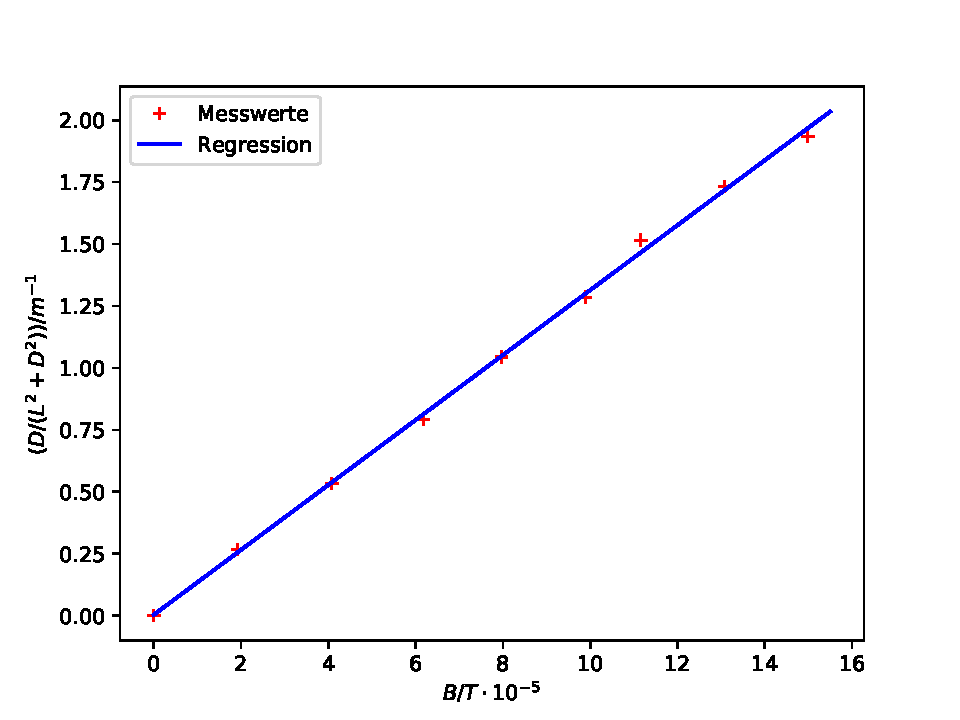
\includegraphics[height=9cm]{plot230e.pdf}
\caption{Bestimmung des Proportionalitätsfaktors für 230V}
\label{fig:230e}
\end{figure}
\begin{figure}
\centering
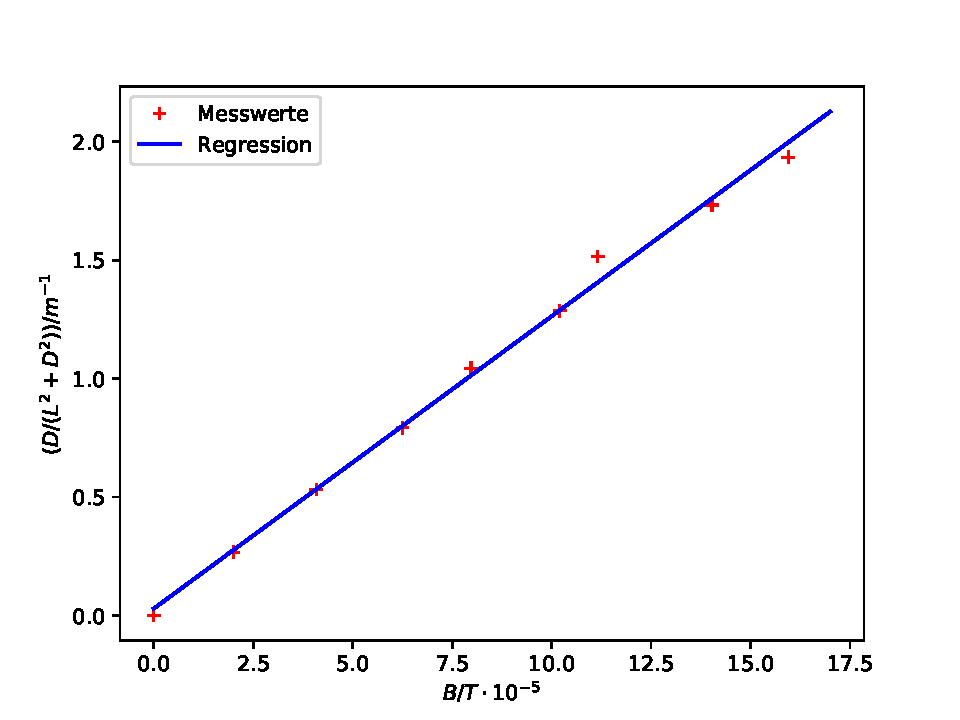
\includegraphics[height=9cm]{plot250e.pdf}
\caption{Bestimmung des Proportionalitätsfaktors für 250V}
\label{fig:250e}
\end{figure}
\begin{figure}
\centering
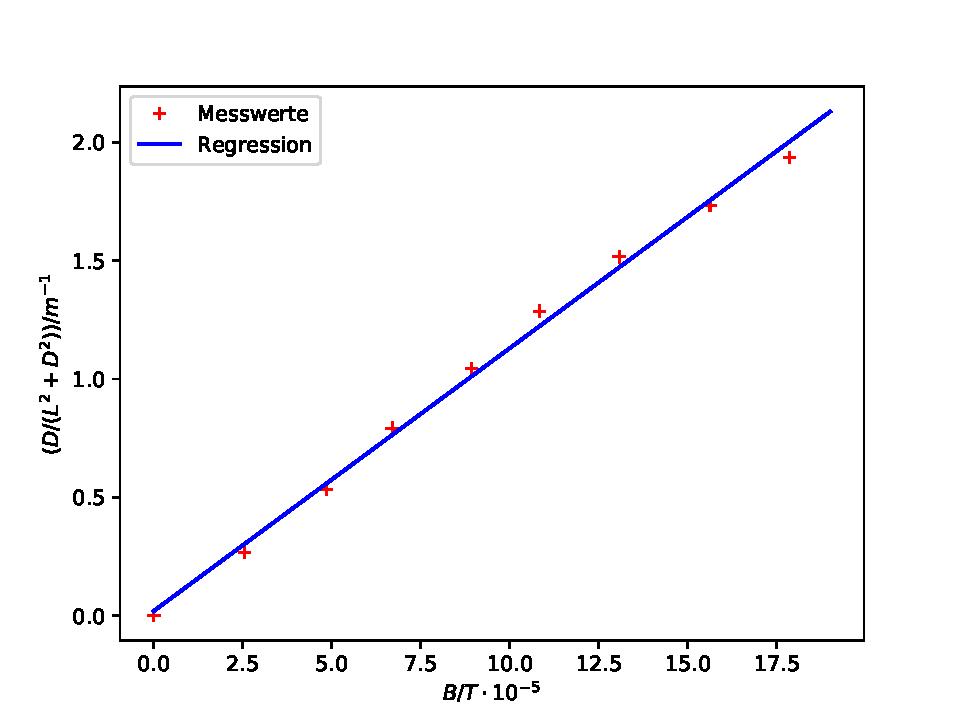
\includegraphics[height=9cm]{plot300e.pdf}
\caption{Bestimmung des Proportionalitätsfaktors für 300V}
\label{fig:300e}
\end{figure}
\begin{figure}
\centering
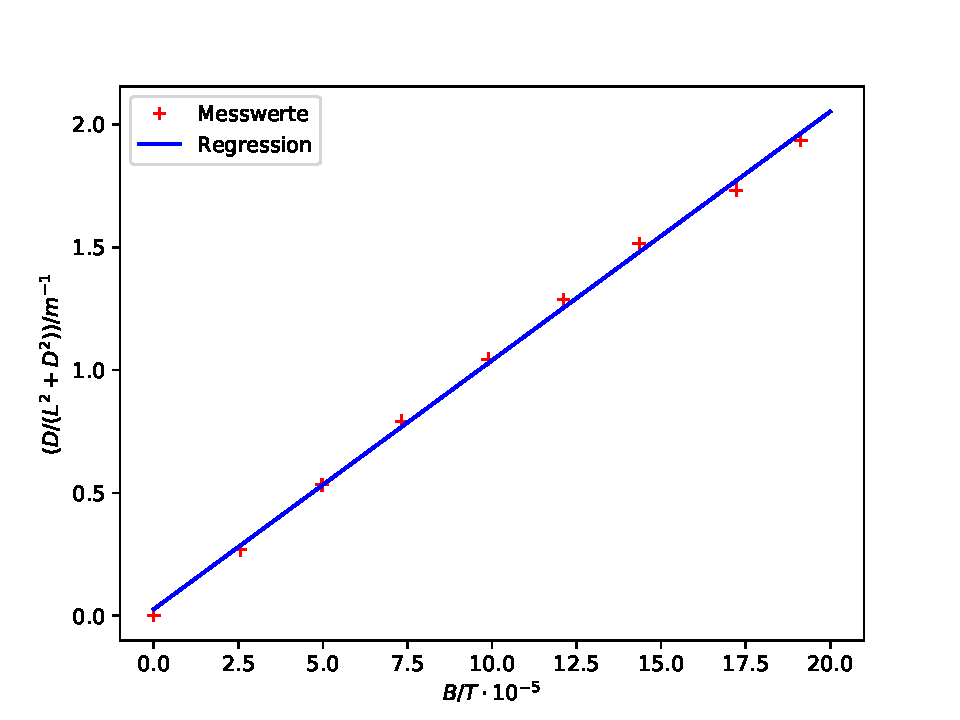
\includegraphics[height=9cm]{plot350e.pdf}
\caption{Bestimmung des Proportionalitätsfaktors für 350V}
\label{fig:350e}
\end{figure}
\begin{figure}
\centering
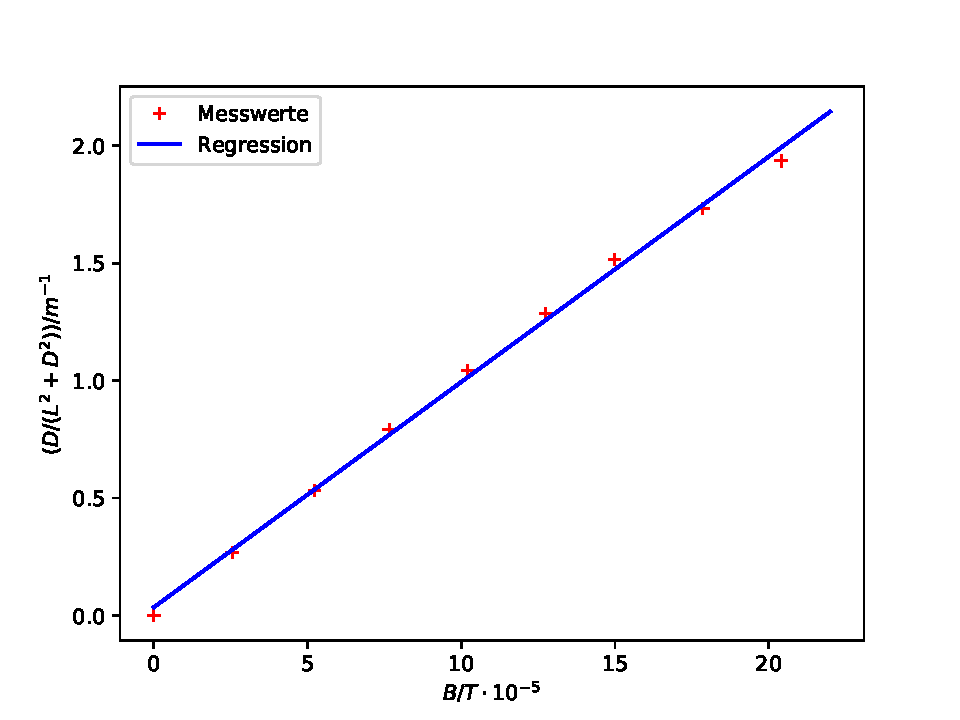
\includegraphics[height=9cm]{plot400e.pdf}
\caption{Bestimmung des Proportionalitätsfaktors für 400V}
\label{fig:400e}
\end{figure}
Aus Formel (\ref{eqn:ladung}) folgt ein linearer Zusammenhang zwischen B und $\sfrac{D}{(L^2+D^2)}$.
Die Formel für die Ausgleichsrechnung lautet:
\begin{equation*}
  \frac{D}{D^2 +L^2}\left(\frac{1}{B}\right) = a\cdot \frac{1}{B}+b
\end{equation*}

Die Parameter, die sich ergeben, sind in Tabelle \ref{tab:a} zu finden.

\begin{table}
  \centering
  \caption{Parameter der Ausgleichsrechnung}
  \label{tab:a}
  \begin{tabular}{c c c}
    \toprule
    $\symup{U_B}/ V$ & $\symup{Steigung\, a/ \frac{1}{mT}}$ & b / $\symup{m^{-1}}$\\
    \midrule
230 & $ (1,311 \pm 0,018)\cdot 10^{4} $ & (0,003\pm 0,016)\\
250 & $ (1,234 \pm 0,034)\cdot 10^{4} $ & (0,030\pm 0,032)\\
300 & $ (1,111 \pm 0,027)\cdot 10^{4} $ & (0,020\pm 0,029)\\
350 & $ (1,013 \pm 0,016)\cdot 10^{4} $ & (0,026\pm 0,019)\\
400 & $ (9,59 \pm 0,18)\cdot 10^{3} $   & (0,035\pm 0,022)\\
\bottomrule
\end{tabular}
\end{table}
%Wird nun über die Steigung gemittelt, ergibt sich für a ein Wert von $(0,792 \pm 0,0972)\cdot {10^-2}$.\\
Aus diesen Steigungen wird nun das Verhältnis von $e_0$ zu $m_0$ bestimmt.
Dafür wird Formel(\ref{eqn:ladung}) verwendet.\\
Daraus folgt:
\begin{align*}
  \frac{D}{D^2+L^2} &= \frac{1}{\sqrt{8U_B}}\sqrt{\frac{e_0}{m_0}}\cdot B\\
  a := \frac{D}{D^2+L^2}\frac{1}{B} &= \frac{1}{\sqrt{8U_B}}\sqrt{\frac{e_0}{m_0}}\\
  \frac{e_0}{m_0} &= 8a^2\cdot U_B .
\end{align*}
Nun kann $\frac{e_0}{m_0}$ bestimmt werden:
\begin{align*}
\left(\frac{e_0}{m_0}\right)_{230} &= 3,162\cdot 10^{11} \, \mathrm{\frac{C}{kg}}\\
\left(\frac{e_0}{m_0}\right)_{250} &= 3,046\cdot 10^{11}  \, \mathrm{\frac{C}{kg}}\\
\left(\frac{e_0}{m_0}\right)_{300} &= 2,962\cdot 10^{11}  \, \mathrm{\frac{C}{kg}}\\
\left(\frac{e_0}{m_0}\right)_{350} &= 2,873\cdot 10^{11}  \, \mathrm{\frac{C}{kg}}\\
\left(\frac{e_0}{m_0}\right)_{400} &= 2,602\cdot 10^{11}   \, \mathrm{\frac{C}{kg}}
\end{align*}
Für das Verhältnis von $e_0$ zu $m_0$ ergibt sich ein Wert von
\begin{equation}
\frac{e_0}{m_0} = (2,929\pm 0,095)\cdot 10^{11} \, \mathrm{\frac{C}{kg}}
  \label{em}
\end{equation}
Der Fehler wurde mit der Formel
\begin{equation*}
\sigma_{\frac{e_0}{m_0}} =  \frac{1}{\sqrt{5}}\cdot \sqrt{\frac{1}{4}\sum _i (x_i - \overline{x_i})}
\end{equation*}
berechnet.\\

%\newpage
Der Spulenstrom $\symup{I_{hor}}$ beträgt $180\, \mathrm{mA}$
Der Inklinationswinkel \varphi  beträgt 71°.
Aus diesen beiden Größen ergibt sich nun die Totalintensität mittels der Formel
\begin{equation*}
  B_{\symup{erd,total}} = \frac{B_{\symup{erd,hor}}}{\symup{cos(\varphi)}}
\end{equation*}
$\symup{B_{erd,hor}}$ ist hierbei gleich $ \symup{B_{Spule}}$.\\
$\symup{B_{Spule}}$ wird mit Formel(\ref{eqn:hh}) bestimmt und beträgt $11,47\, \mathrm{\mu T}$.
Somit ergibt sich
\begin{equation*}
  B_{erd,total} = 35,23 \, \mathrm{\mu T}
\end{equation*}

\section{Diskussion}
\subsection{Ablenkung des Elektronenstrahls im E-Feld}

Das im ersten Aufgabenteil bestimmte C aus Formel (\ref{eqn:a}) sollte mit der Steigung aus Abbildung \ref{fig:empfvsu} übereinstimmenn.
Die ermittelten Größen lauten:
\begin{align*}
  C_T&= 0,219\, \mathrm{m} \\
  a = C_M &= 0,356\,\mathrm{m}
\end{align*}
Die Abweichung beträgt 62,56\%
und wurde mit der Formel
\begin{equation}
  \symup{p_c} = \left|\frac{C_{Messung} - C_{Theorie}}{C_{Theorie}}\right|
  \label{eqn:abw}
\end{equation}
berechnet.\\
Die Fits für die bestimmung der Empfindlichkeiten aus den Abbildungen \ref{fig:230b} - \ref{fig:400b} sind recht genau
und beinhalten keine größeren Abweichungen.
Auch der daraus resultierende Fit in Abbildung \ref{fig:empfvsu} weist nur kleinere Abweichungen auf.
%Die Werte für die Beschleunigungsspannungen von 230V und 250V liegen nicht ganz auf der Geraden
Somit sind die Fehler der bestimmten Parameter auch eher gering.
Der bestimmte Theoriewert hat eine Fehlerbelastung, da über den Abstand der beiden Platten gemittelt werden musste.
Das kann die Abweichung zum Teil erklären.

Im zweiten Teil des Versuches wurde die Frequenz der Sinunsspannung und der Scheitelwert bestimmt.
Die ermittelte Frequenz $(80,10 \pm 0,39)\, \mathrm{Hz}$ und der Scheitelwert $(11,10 \pm 0,80)\, \mathrm{V}$ weisen keine großen Fehler auf,
sodass davon ausgegangen werden kann, dass es keine größeren Fehlerquellen gab.
\subsection{Ablenkung des Elektronenstrahls im B-Feld}
Ziel dieses Versuchsteils ist die Bestimmung des Verhältnis von $\symup{e_0}$ zu $\symup{m_0}$.

Die Verhältnisse betragen
\begin{align*}
\frac{e_0}{m_0}_{Messung} &= (2,929\pm 0,095)\cdot 10^{11} \, \mathrm{\frac{C}{kg}} \\
\frac{e_0}{m_0}_{Theorie} &= 1,75\cdot 10^{11}\,\mathrm{\frac{C}{kg}}
\end{align*}
\cite{em}

Es ergibt sich eine Abweichung von 66,86\%.
Sie wurde mit Formel
\begin{equation*}
\symup{p_{\frac{e_0}{m_0}}} = \left|\frac{\left(\frac{e_0}{m_0}\right)_{Messung} -
\left(\frac{e_0}{m_0}\right)_{Theorie}}{\left(\frac{e_0}{m_0}\right)_{Theorie}}\right|
\end{equation*}
bestimmt.
Die Ausgleichsgeraden aus den Abbildungen \ref{fig:230e} - \ref{fig:400e}
weisen keine größeren Abweichungen zu den Werten auf.
Somit ist die Fehlerbelastung der Parameter eher gering.\\
Kleinere Abweichungen können damit erklärt werden,
dass der gemessene Strom zu den einzelnen Abständen sehr ungenau ist da die Abstände per Augenmaß eingestellt wurden.
Der Leuchtpunkt, nach dem sich dies orientierte war nicht ganz scharf einstellbar.
Eine weitere Fehlerquelle ist das Amperemeter.
Beim umschalten in andere Größenordnungen, wurde nicht genau der selben Wert angezeigt.

Im nächsten Teil wurde das Erdmagnetfeld bestimmt.
\begin{align*}
  \symup{B_{erd,total(Messung)}} &= 35,23 \, \mathrm{\mu T}\\
  \symup{B_{erd,total(Theorie)}} &= 44\, \mathrm{\mu T}
\end{align*}
 \cite{on2}

Mit Formel
\begin{equation*}
  \symup{p_B} = \left|\frac{B_{Messung} - B_{Theorie}}{B_{Theorie}}\right|
\end{equation*}
ergibt sich eine Abweichung von 19,93\%
Für die Bestimmung des Erdmagnetfeldes, musste der Inklinationswinkel bestimmt werden.
Der Kompass, mit dem dies durchgeführt wurde  war sehr ungenau.
Die Nadel bewegte sich nicht ganz frei und steckte leicht fest.
Außerdem schwankte der Wert des Kompass, mit dem der Versuchsaufbau nach Norden ausgerichtet wurde.
Somit ist nicht ganz sichergestellt, dass der Aufbau exakt nach Norden ausgerichtet war.
